\chapter{Aufgabe 6}
\section{Aufgabe 6.1}

\begin{wrapfigure}[13]{r}{.3\textwidth}
	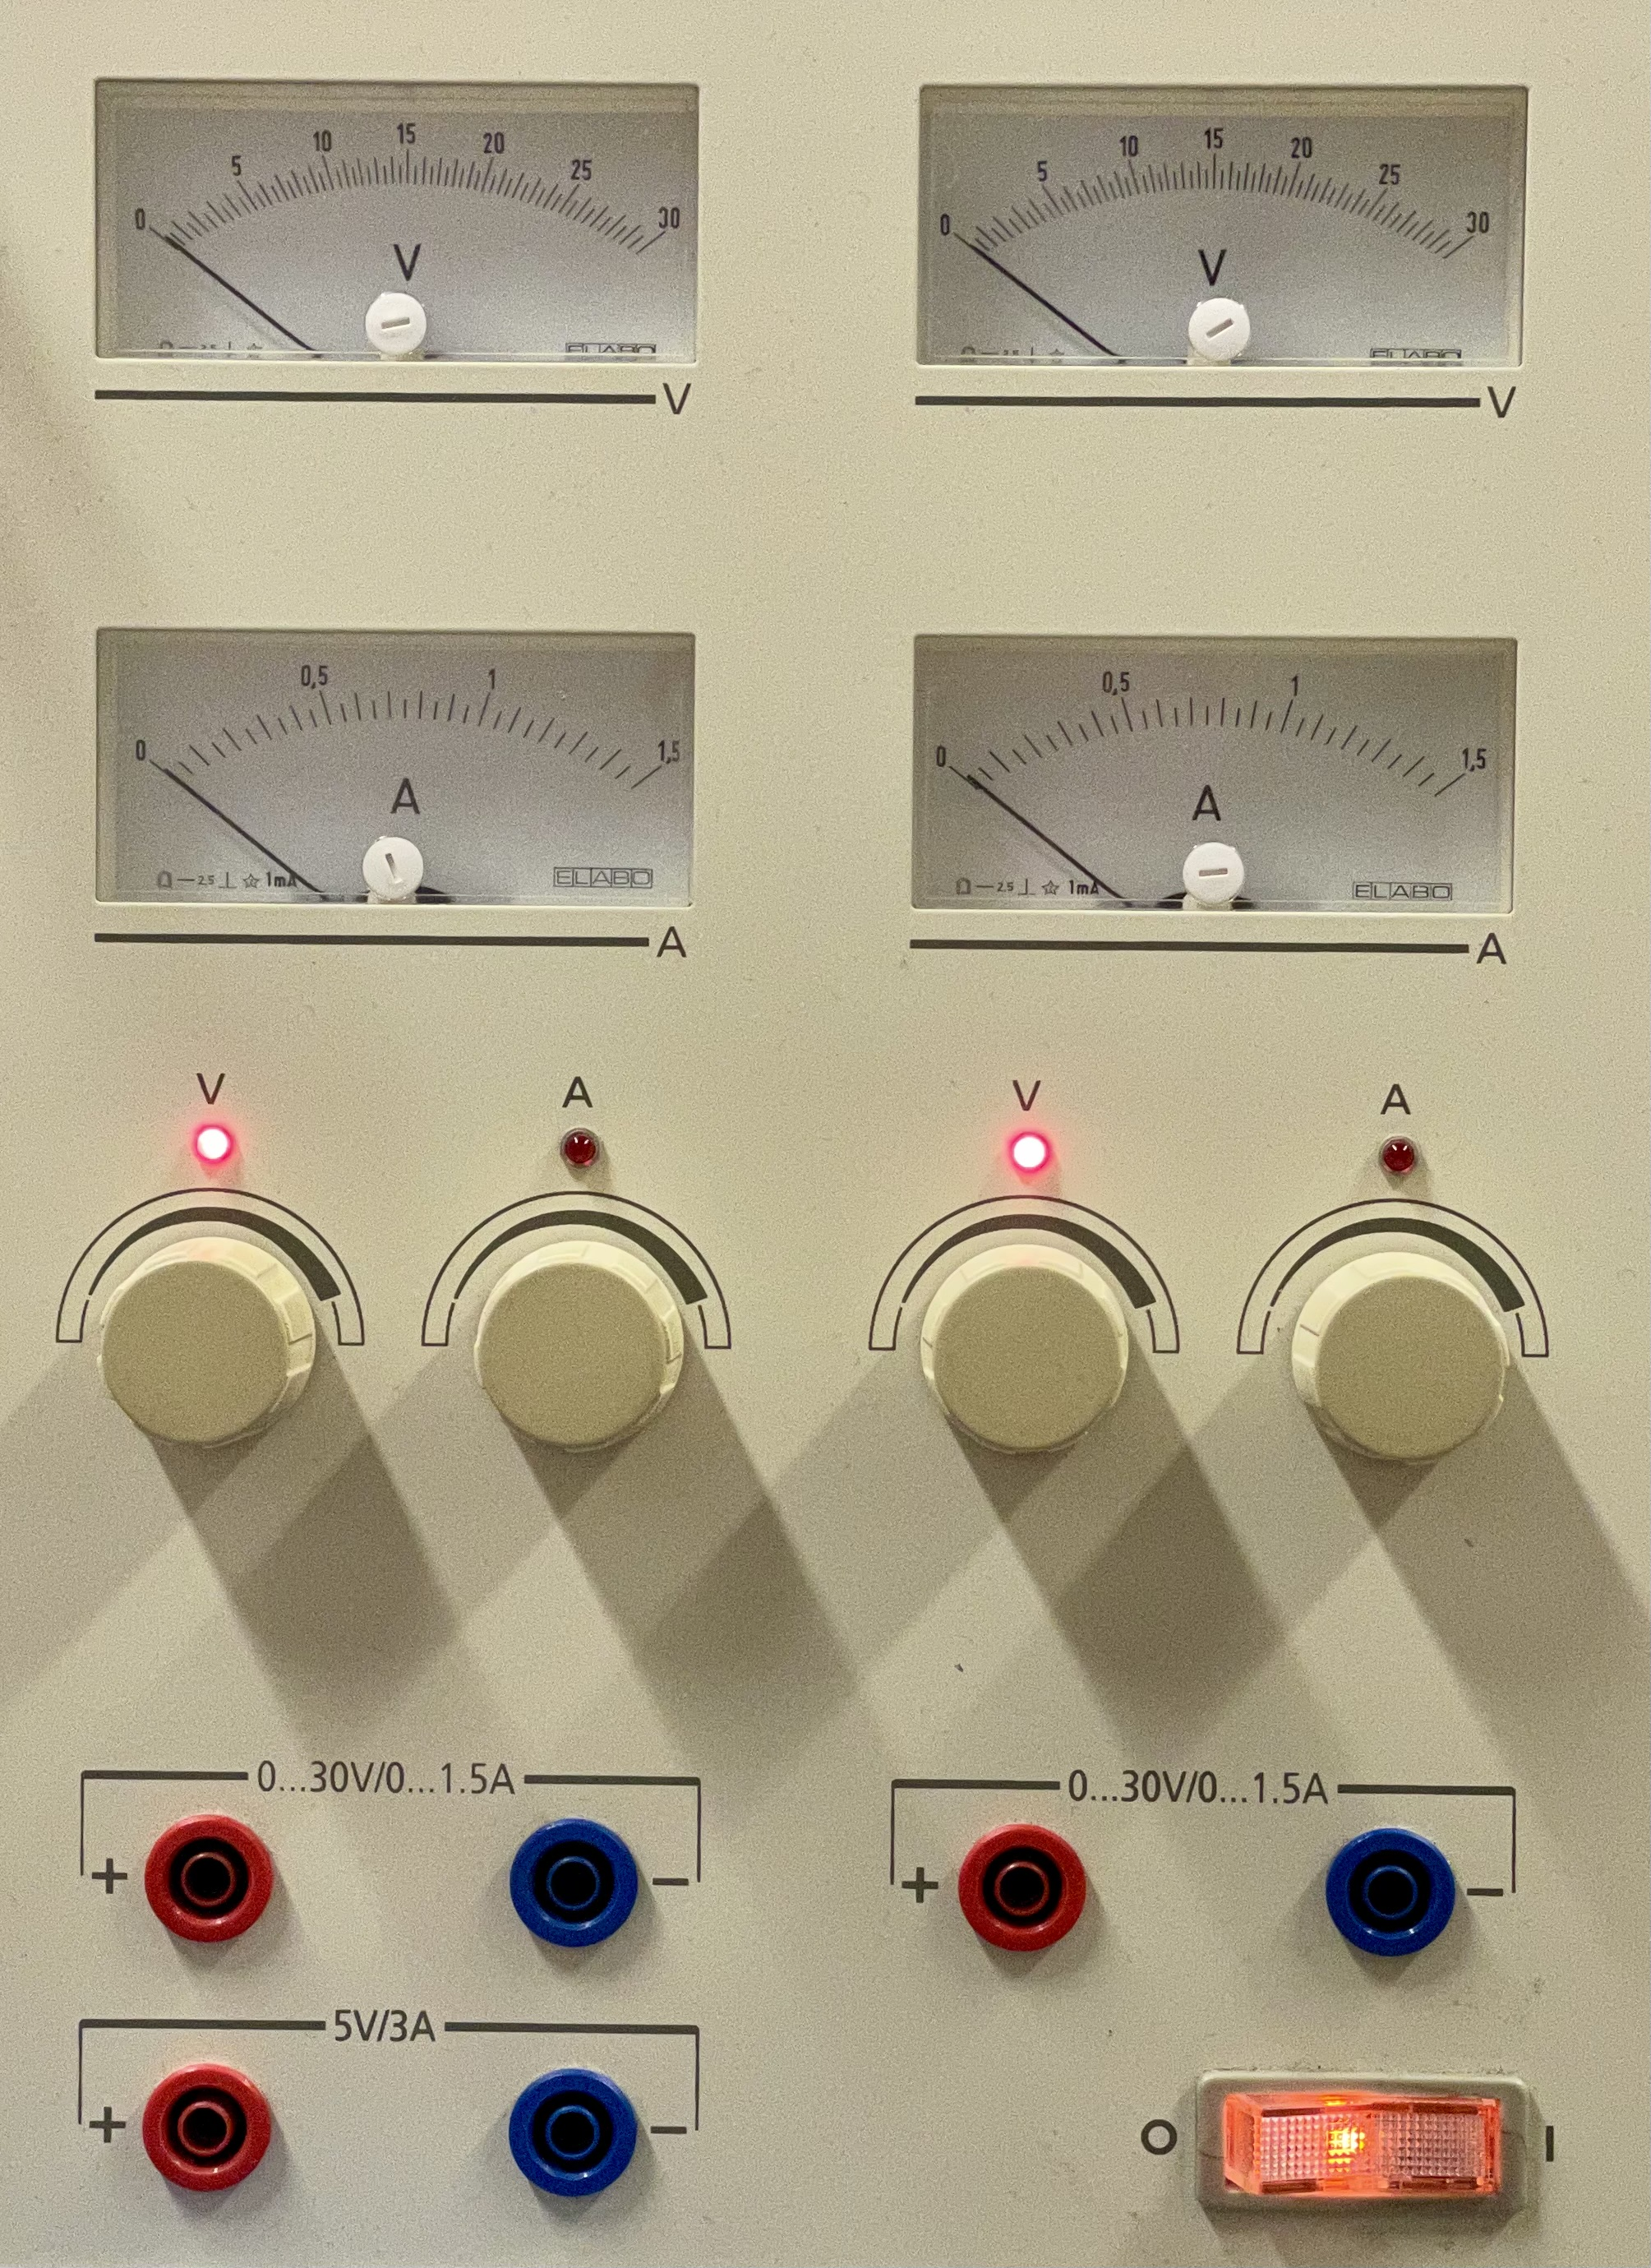
\includegraphics[width=.3\textwidth]{task6-1-0.JPG}
	\caption{Netzteil}
	\label{task6-1-0}
\end{wrapfigure}

\paragraph{Aufgabenstellung}
Entfernen Sie alle Kabel vom Netzteil, schalten Sie das Netzteil an und stellen Sie das Netzteil entsprechend den Vorgaben ein!

\paragraph{Durchführung}
Zu beginn befinden sich keine Kabel am Netzteil und es wird eingeschaltet (Abb. \vref{task6-1-0}). Nach dem Einschalten kann die Spannung eingestellt werden. Links sind $8V$ und rechts $5V$ einzustellen (Abb \vref{task6-1-1}). Um die Stromstärke einzustellen, müssen jeweils beide Buchsen der Netzteile kurzgeschlossen werden. Links werden $1A$ und rechts $50mA$ eingestellt (Abb. \vref{task6-1-2}).

\begin{figure}
	\begin{minipage}[c]{0.5\textwidth}
		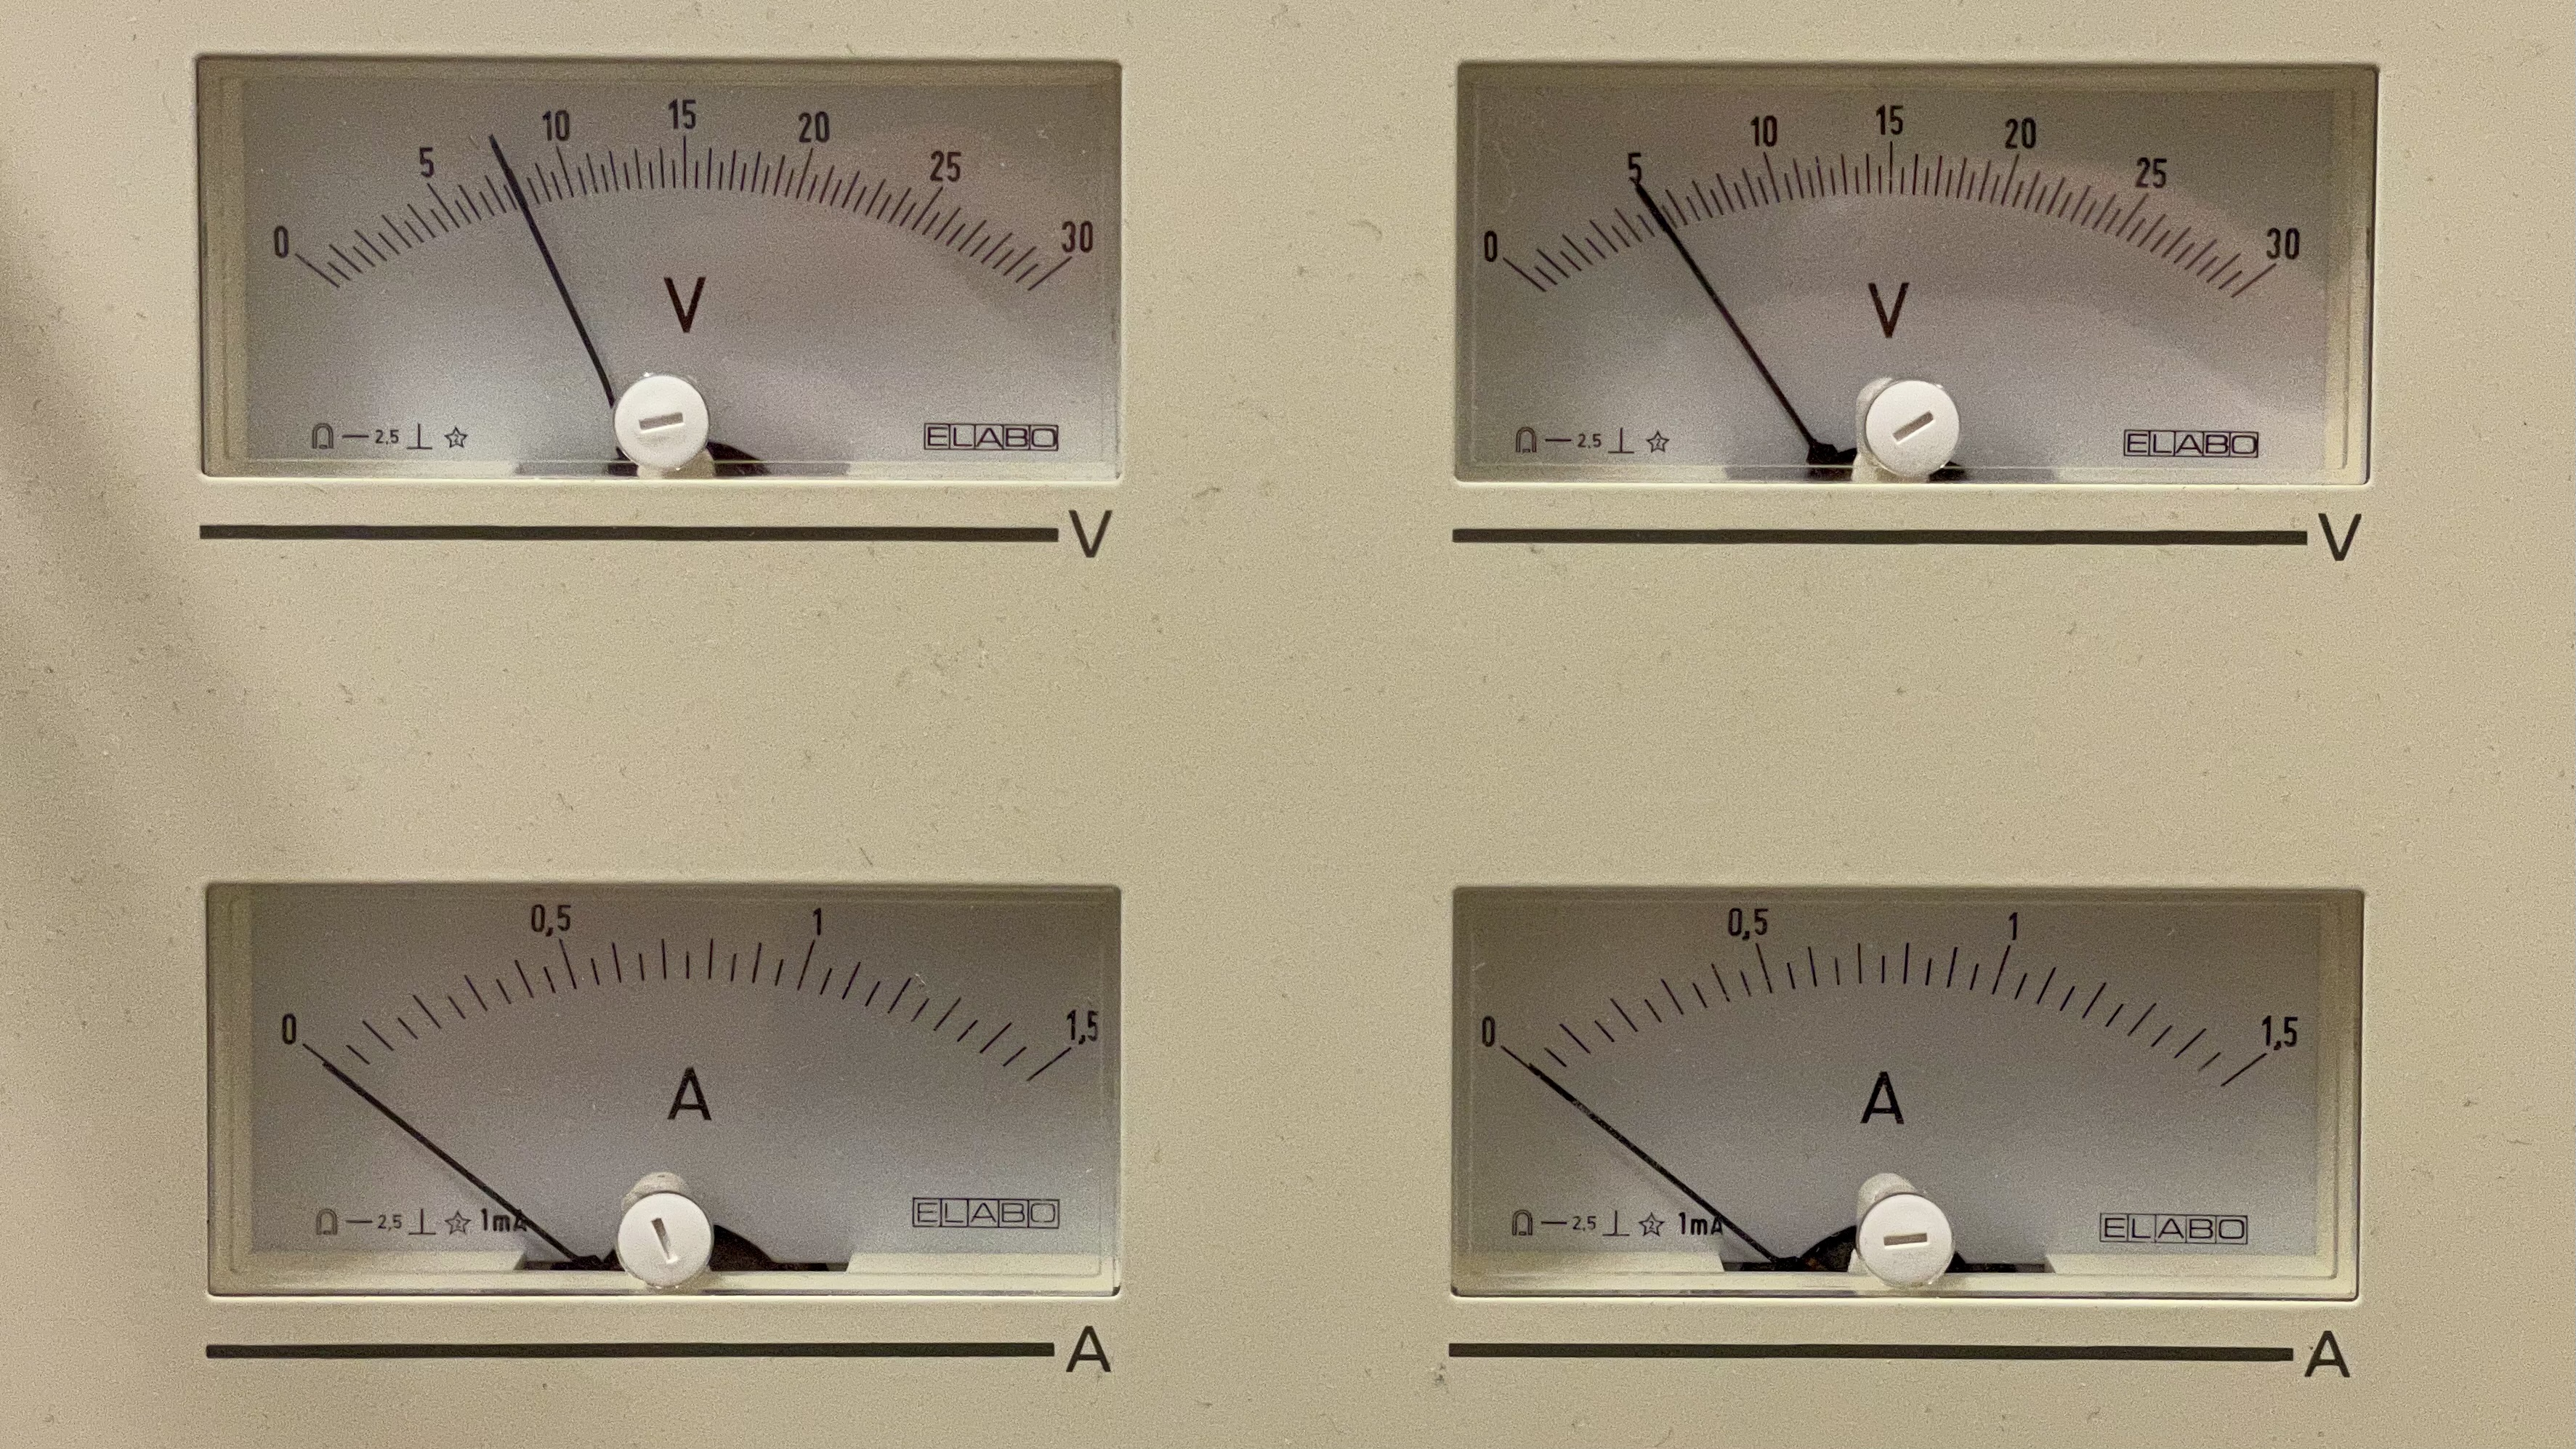
\includegraphics[width=\textwidth]{task6-1-1.JPG}
		\caption{Einstellen der Spannung}
		\label{task6-1-1}
	\end{minipage}
	\hfill
	\begin{minipage}[c]{0.44\textwidth}
		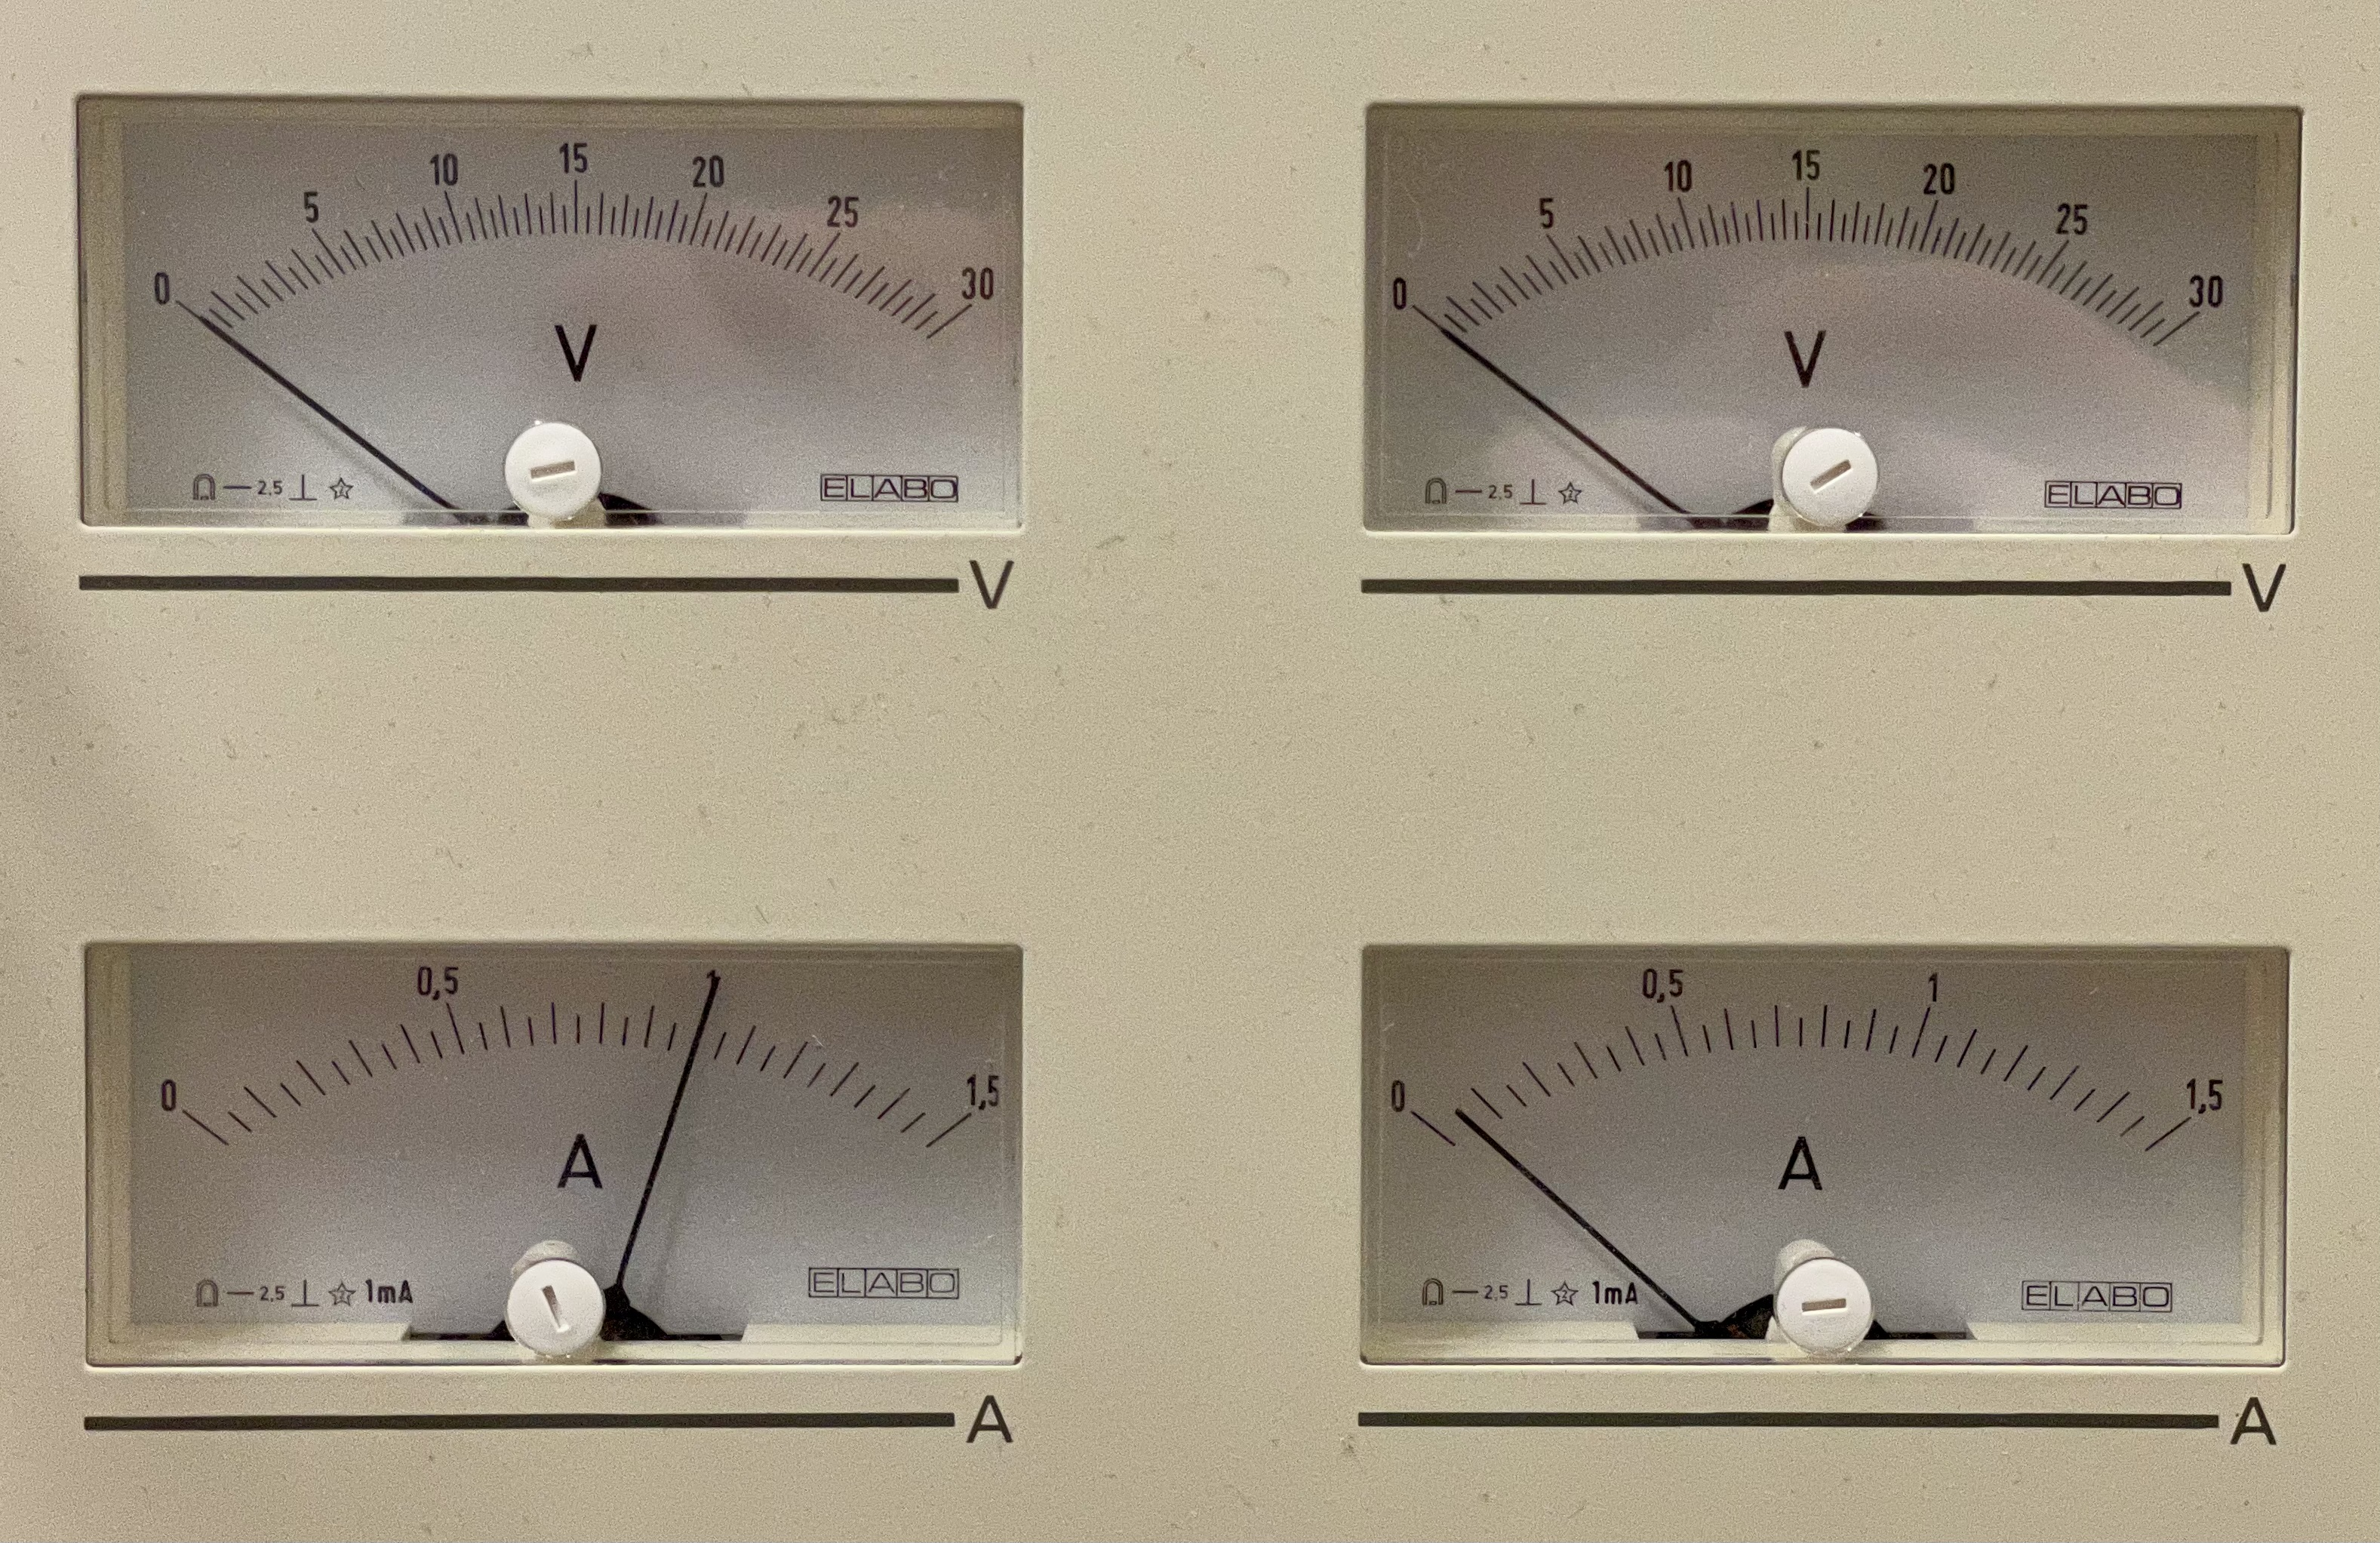
\includegraphics[width=\textwidth]{task6-1-2.JPG}
		\caption{Einstellen der Stromstärke}
		\label{task6-1-2}
	\end{minipage}
\end{figure}

\section{Aufgabe 6.2}
\paragraph{Aufgabenstellung}
Ermitteln Sie die Abweichung zwischen den digitalen Multimetern und den eingebauten analogen Anzeigen der Spannungsversorgung!

\paragraph{Durchführung}
Um die Spannung zu messen, wird das linke Multimeter über die Buchsen COM (Schwarz) und V (Rot) mit dem rechten Netzteil verbunden.

\begin{figure}
	\begin{minipage}[c]{0.49\textwidth}
		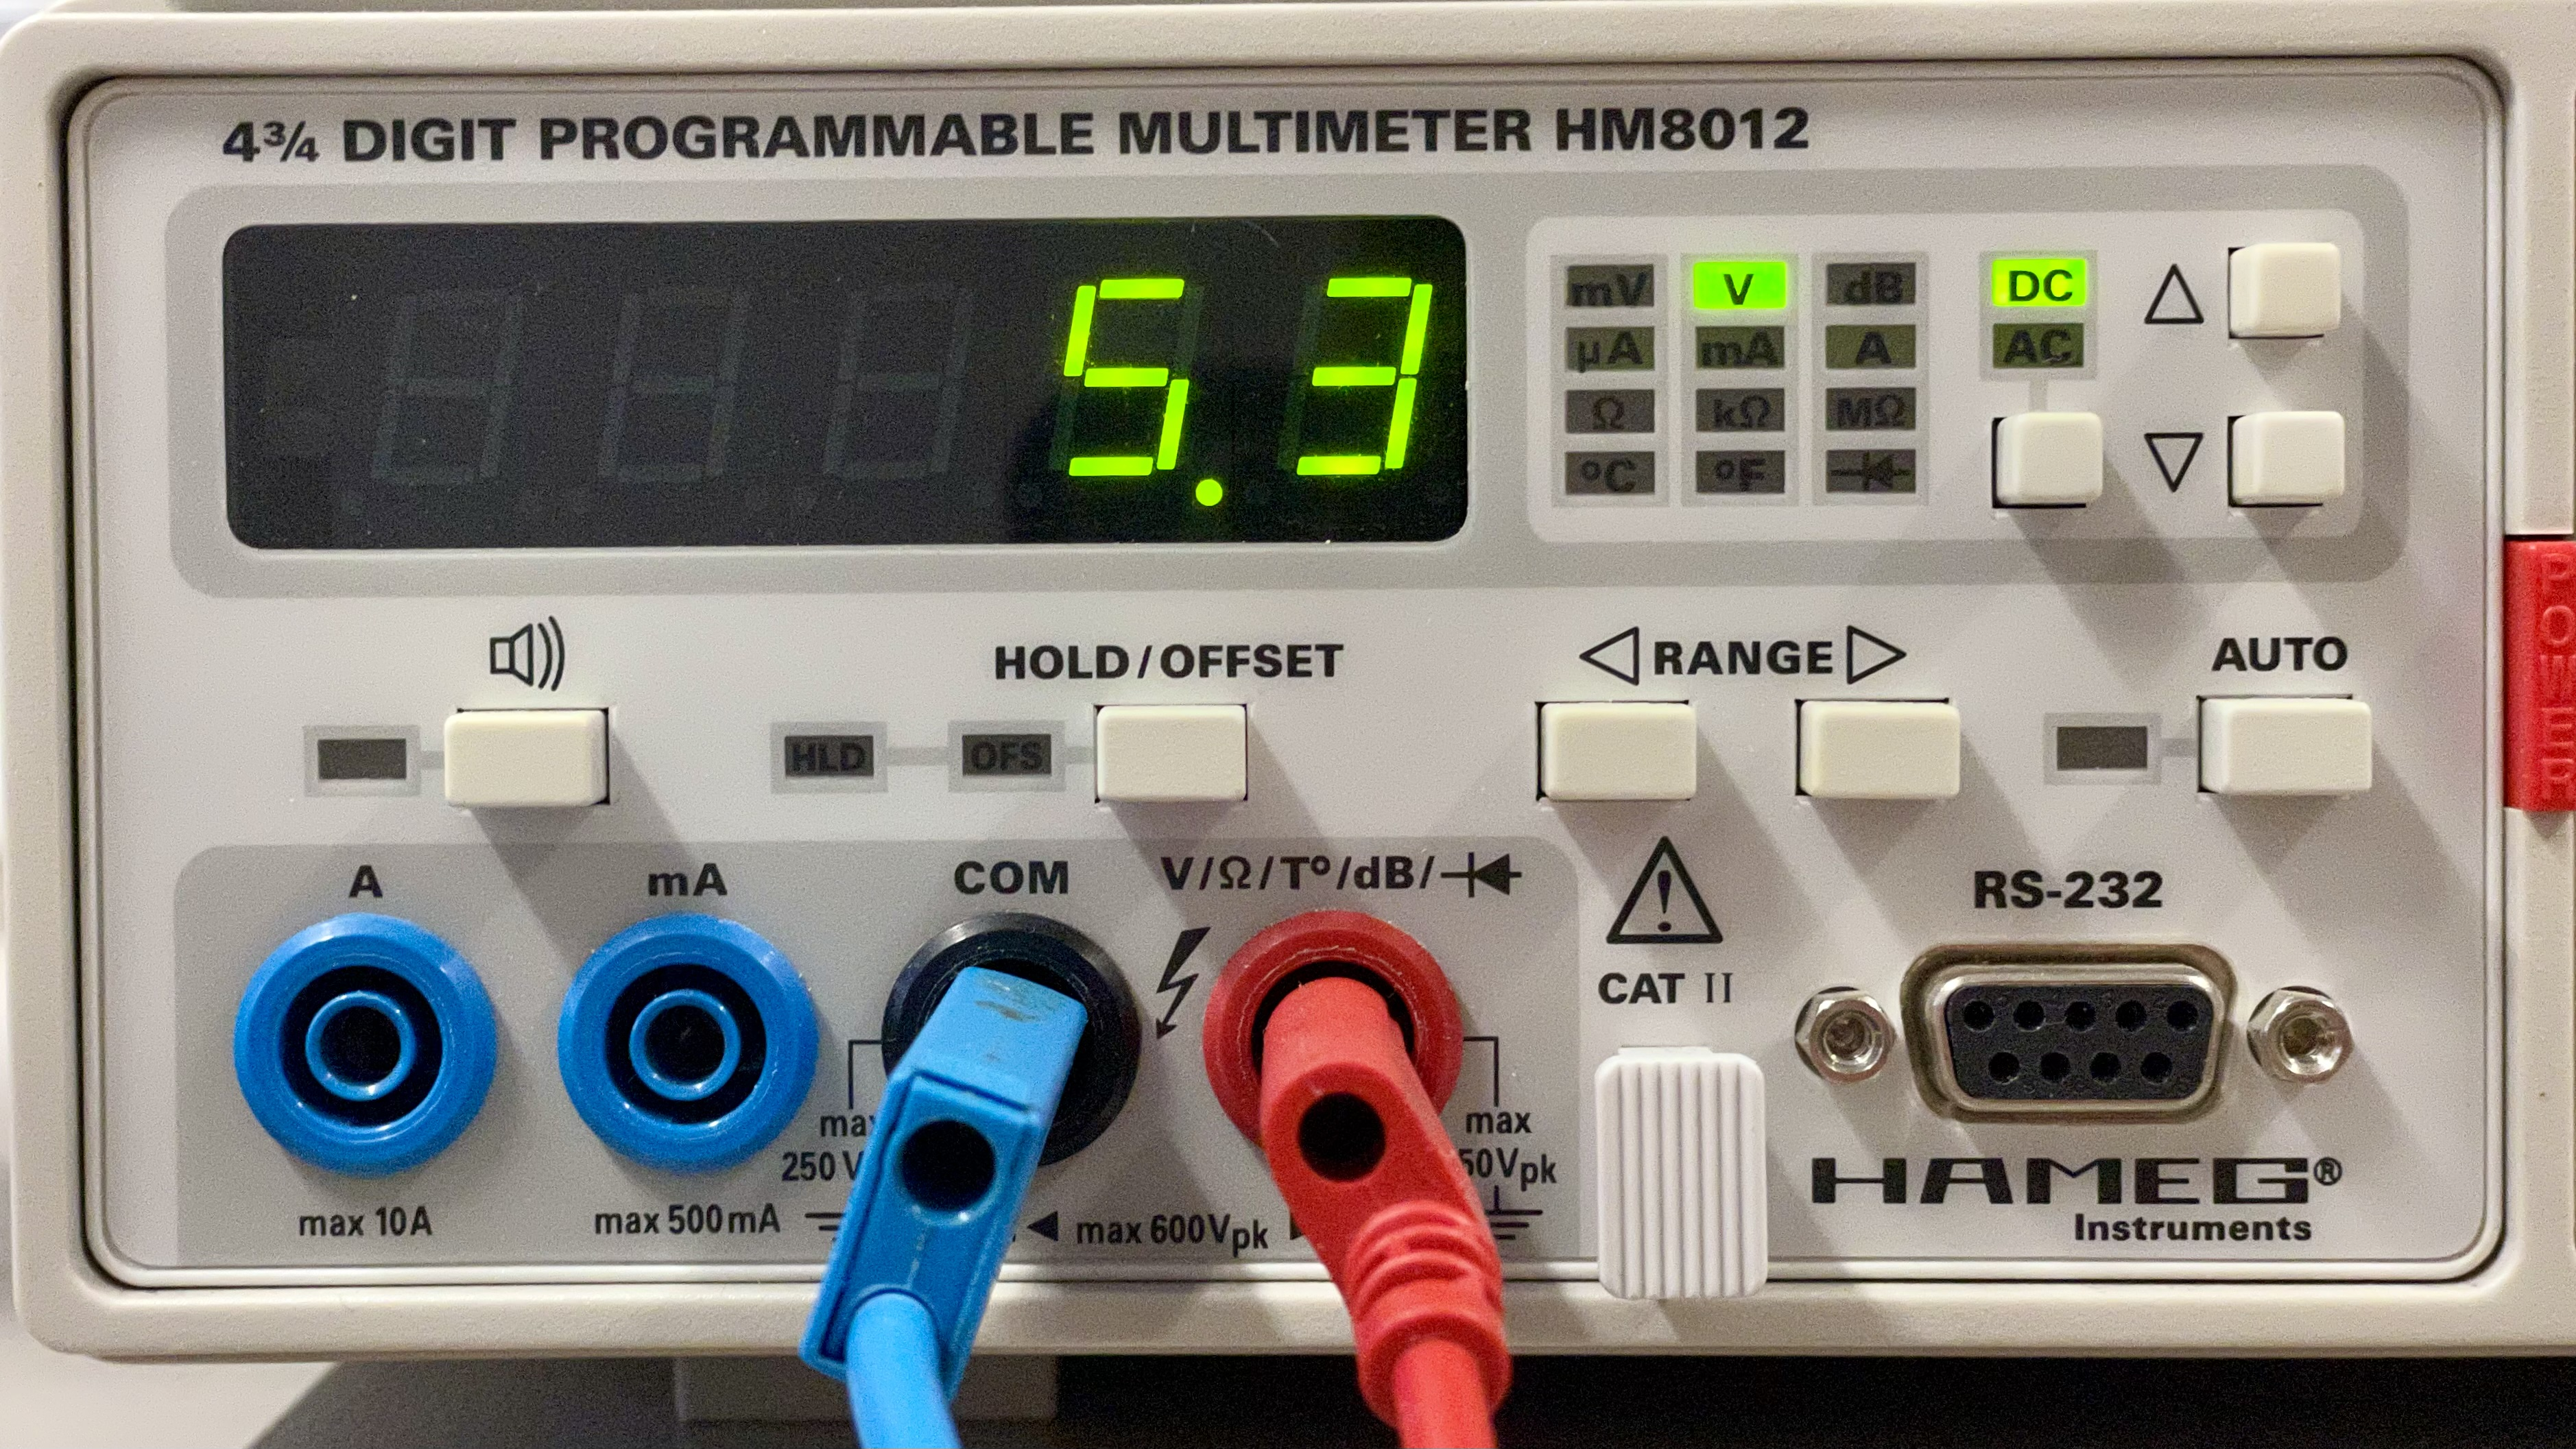
\includegraphics[width=\textwidth]{task6-2-0.JPG}
		\caption{Messen der Spannung}
		\label{task6-2-0}
	\end{minipage}
	\begin{minipage}[c]{0.49\textwidth}
		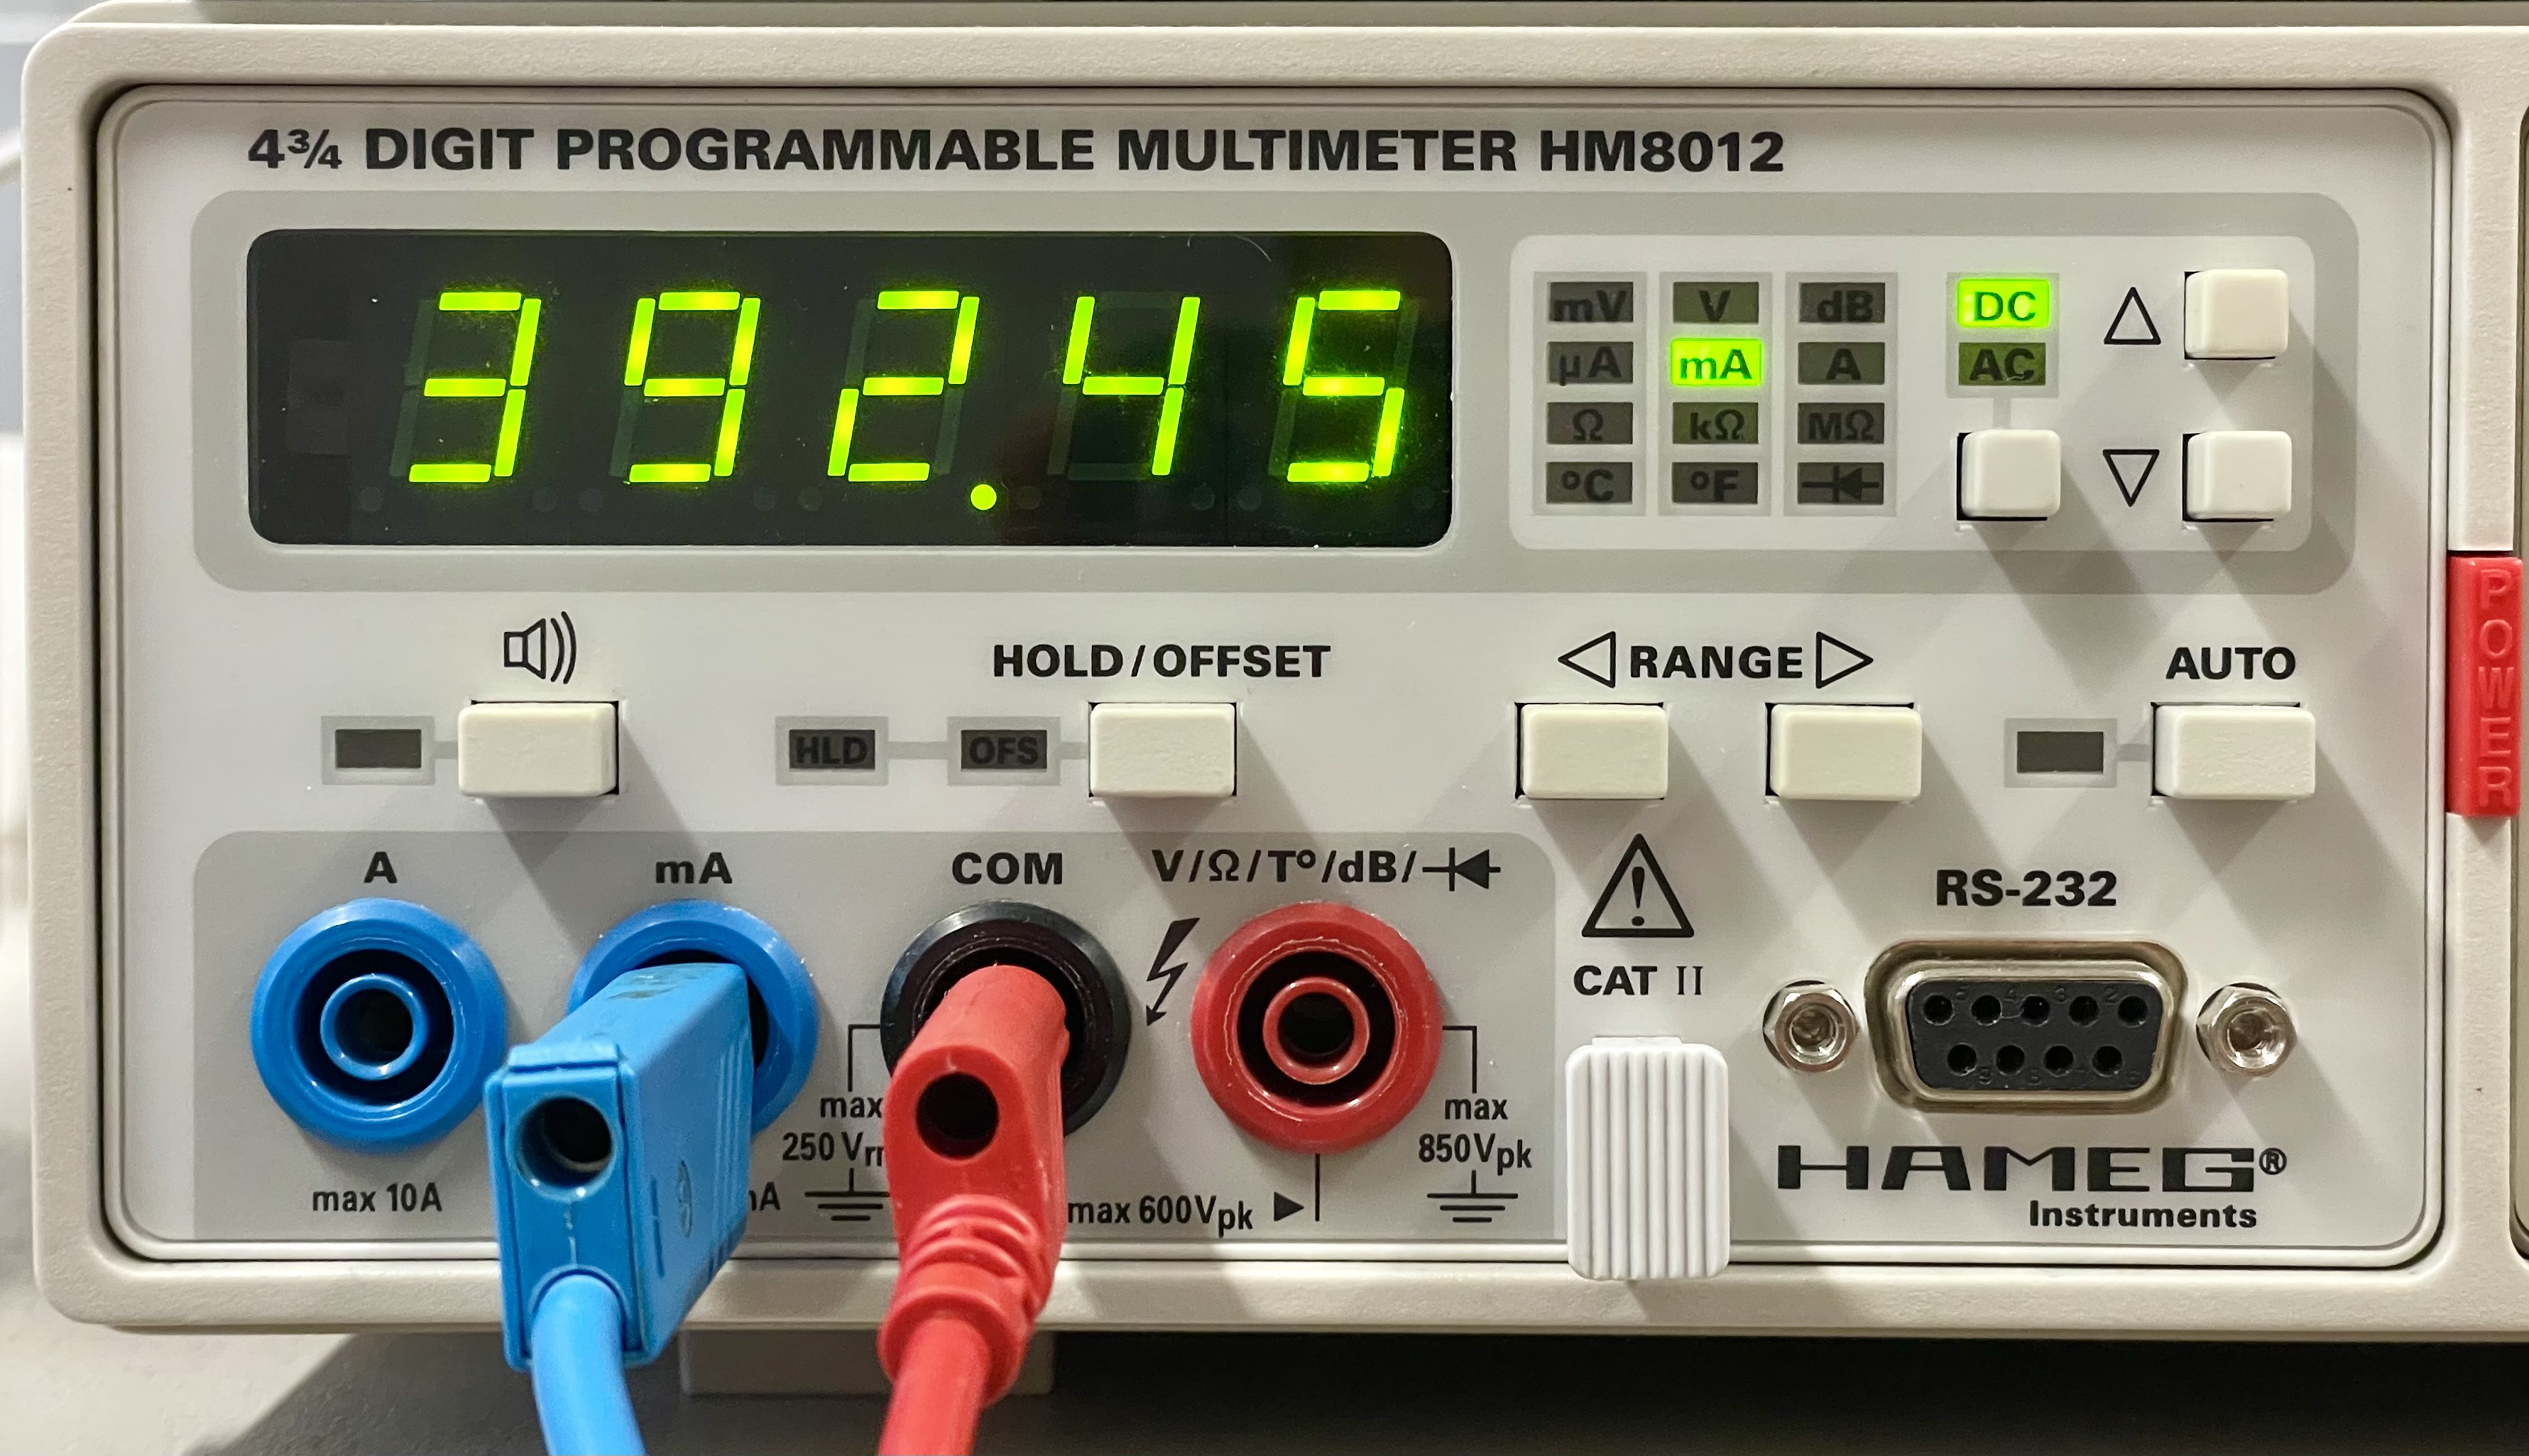
\includegraphics[width=\textwidth]{task6-2-1.JPG}
		\caption{Messen der Stromstärke}
		\label{task6-2-1}
	\end{minipage}
\end{figure}